% Тип документа
\documentclass[a4paper,14pt]{extarticle}

% Шрифты, кодировки, символьные таблицы, переносы
\usepackage{cmap}
\usepackage[T2A]{fontenc}
\usepackage[utf8x]{inputenc}
\usepackage[russian]{babel}
\usepackage[table]{xcolor}
% Это пакет -- хитрый пакет, он нужен но не нужен
\usepackage[mode=buildnew]{standalone}

\usepackage
	{
		% Дополнения Американского математического общества (AMS)
		amssymb,
		amsfonts,
		amsmath,
		amsthm,
		physics,
		% misccorr,
		% 
		% Графики и рисунки
		wrapfig,
		graphicx,
		subcaption,
		float,
		tikz,
		tikz-3dplot,
		caption,
		csvsimple,
		color,
		booktabs,
		pgfplots,
		pgfplotstable,
		geometry,
		% 
		% Таблицы, списки
		array,
		makecell,
		multirow,
		indentfirst,
		%
		% Интегралы и прочие обозначения
		ulem,
		esint,
		esdiff,
		% 
		% Колонтитулы
		fancyhdr,
	}  

\usepackage{xcolor}
\usepackage{hyperref}

 % Цвета для гиперссылок
\definecolor{linkcolor}{HTML}{000000} % цвет ссылок
\definecolor{urlcolor}{HTML}{799B03} % цвет гиперссылок
 
\hypersetup{pdfstartview=FitH,  linkcolor=linkcolor,urlcolor=urlcolor, colorlinks=true}
% Обводка текста в TikZ
\usepackage[outline]{contour}

% Увеличенный межстрочный интервал, французские пробелы
\linespread{1.1} 
\frenchspacing 

 
\usetikzlibrary
	{
		decorations.pathreplacing,
		decorations.pathmorphing,
		patterns,
		calc,
		scopes,
		arrows,
		fadings,
		through,
		shapes.misc,
		arrows.meta,
		3d,
		quotes,
		angles,
		babel
	}

\usepgfplotslibrary{units}

% const прямым шрифтом
\newcommand\ct[1]{\text{\rmfamily\upshape #1}}
\newcommand*{\const}{\ct{const}}
\renewcommand*{\epsilon}{\varepsilon}

\usepackage[europeanresistors,americaninductors]{circuitikz}

% Style to select only points from #1 to #2 (inclusive)
\pgfplotsset{select/.style 2 args={
    x filter/.code={
        \ifnum\coordindex<#1\def\pgfmathresult{}\fi
        \ifnum\coordindex>#2\def\pgfmathresult{}\fi
    }
}}

\usepackage{array}
\usepackage{pstool}

%%%%%%%%%%%%%%%%%%%%%%%%%%%%%%%%%%%%%%%%%%%%%%%%%
\makeatletter
\newif\if@gather@prefix 
\preto\place@tag@gather{% 
  \if@gather@prefix\iftagsleft@ 
    \kern-\gdisplaywidth@ 
    \rlap{\gather@prefix}% 
    \kern\gdisplaywidth@ 
  \fi\fi 
} 
\appto\place@tag@gather{% 
  \if@gather@prefix\iftagsleft@\else 
    \kern-\displaywidth 
    \rlap{\gather@prefix}% 
    \kern\displaywidth 
  \fi\fi 
  \global\@gather@prefixfalse 
} 
\preto\place@tag{% 
  \if@gather@prefix\iftagsleft@ 
    \kern-\gdisplaywidth@ 
    \rlap{\gather@prefix}% 
    \kern\displaywidth@ 
  \fi\fi 
} 
\appto\place@tag{% 
  \if@gather@prefix\iftagsleft@\else 
    \kern-\displaywidth 
    \rlap{\gather@prefix}% 
    \kern\displaywidth 
  \fi\fi 
  \global\@gather@prefixfalse 
} 
\newcommand*{\beforetext}[1]{% 
  \ifmeasuring@\else
  \gdef\gather@prefix{#1}% 
  \global\@gather@prefixtrue 
  \fi
} 
\makeatother
%%%%%%%%%%%%%%%%%%%%%%%%%%%%%%%%%%%%%%%%%%%%%%%%%

\geometry		
	{
		left			=	2cm,
		right 			=	2cm,
		top 			=	3cm,
		bottom 			=	3cm,
		bindingoffset	=	0cm
	}

%%%%%%%%%%%%%%%%%%%%%%%%%%%%%%%%%%%%%%%%%%%%%%%%%%%%%%%%%%%%%%%%%%%%%%%%%%%%%%%

	%применим колонтитул к стилю страницы
\pagestyle{fancy} 
	%очистим "шапку" страницы
\fancyhead{} 
	%слева сверху на четных и справа на нечетных
\fancyhead[R]{\labauthors} 
	%справа сверху на четных и слева на нечетных
\fancyhead[L]{Отчёт по лабораторной работе №\labnumber} 
	%очистим "подвал" страницы
\fancyfoot{} 
	% номер страницы в нижнем колинтуле в центре
\fancyfoot[C]{\thepage} 

%%%%%%%%%%%%%%%%%%%%%%%%%%%%%%%%%%%%%%%%%%%%%%%%%%%%%%%%%%%%%%%%%%%%%%%%%%%%%%%

\renewcommand{\contentsname}{Оглавление}

\usepackage{tocloft}
% \renewcommand{\cftpartleader}{\cftdotfill{\cftdotsep}} % for parts
% \renewcommand{\cftsectiondotsep}{\cftdotsep}% Chapters should use dots in ToC
\renewcommand{\cftsecleader}{\cftdotfill{\cftdotsep}}
%\renewcommand{\cftsecleader}{\cftdotfill{\cftdotsep}} % for sections, if you really want! (It is default in report and book class (So you may not need it).
% ---------
% \newcommand{\cftchapaftersnum}{.}%
% \usepackage{titlesec}
% \titlelabel{\thetitle.\quad}
\usepackage{secdot}
\sectiondot{subsection}
\newcommand{\rot}{\operatorname{rot}}
\begin{document}

\def\labauthors{Карусевич А.А., Шиков А.П.}
\def\labgroup{440}
\def\labnumber{2}
\def\labtheme{Электромагнитное экранирование}
\begin{titlepage}

\begin{center}

{\small\textsc{Нижегородский государственный университет имени Н.\,И. Лобачевского}}
\vskip 1pt \hrule \vskip 3pt
{\small\textsc{Радиофизический факультет. Кафедра Электродинамики.}}

\vfill

{\Large Отчет по лабораторной работе №\labnumber\vskip 12pt\bfseries \labtheme}
	
\end{center}

\vfill
	
\begin{flushright}
	{Выполнили студенты \labgroup\ группы\\ \labauthors}%\vskip 12pt Принял:\\ Менсов С.\,Н.}
\end{flushright}
	
\vfill
	
\begin{center}
	Нижний Новгород, \the\year
\end{center}

\end{titlepage}



\newpage

{\bfseries Цель работы:} 
Экспериментальное наблюдение явления экранирования переменного магнитного поля металлическими оболочками и выяснение роли основных физических факторов (свойств материала экрана, а именно - проводимости и магнитной проницаемости; толщины его стенок; частоты поля), определяющих степень проникновения поля через экран, а также теоретический расчет экранирующих свойств металлических оболочек на простой модели и сопоставление экспериментальных и теоретических данных.

\section{Теоретическая часть}
\subsection{Введение}

Под электромагнитным экранированием понимается изоляция некоторой области пространства от проникновения электромагнитных полей, существующих в соседних областях. В статических или переменных квазистационарных полях (которым соответствуют длины волн, много большие характерных размеров используемых приборов и устройств) такая изоляция осуществляется обычно с помощью замкнутых металлических оболочек - экранов. 

Общей физической причиной ослабления поля внутри экрана является то обстоятельство, что наведенные в нем внешнем полем токи (или заряды) создают во внутренней области поле, противоположное внешнему. В результате суммарное поле в этой области, складывающееся из полей внешних и наведенных источников, уменьшается. 
% Если $\lambda_0\gg l$, где $\lambda_0$ -- длина волны экранируемого поля, $l$ -- характерный размер экранируемой области, то такая изоляция осуществляется обычно с помощью замкнутых металлических оболочек -- экранов.} переменного магнитного поля стальными ($\sigma \simeq 0.7\cdot 10^{17} \,c^{-1}, \mu \sim 10^2 \divisionsymbol 10^3 $ при $H \sim 10$ эрстед) и латунными ($\sigma \simeq 1.5\cdot 10^{17}\, c^{-1}, \mu \cong 1$) цилиндрическими экранами на частотах экранируемого поля $20\divisionsymbol10^4$ Гц.  

% Внутренние размеры всех экранов одинаковы (высота и радиус основания $h=R$ = 5 см), а толщина стенок различна ($d=$ 0.2 см, 0.5 см, 1 см). 

% Строгий аналитический расчет экранирования цилиндрическими замкнутыми экранами невозможен. Простыми моделями, допускающими точное решение задачи в аналитических функциях являются, например, модель плоского, цилиндрического и сферического слоя.

% Среди этих моделей замкнутый экран можно описать только сферическим слоем. Кроме того, характерные размеры используемого экрана малы по сравнению с длиной волны экранируемого поля ($\lambda_0\sim10$ км $\Rightarrow h,D\ll\lambda_0$). Поэтому адекватным выбором для качественных оценок является именно сферическая модель. Для того, чтобы получить близкие и количественные результаты, логично взять для сферической модели же объем внутренней полости, что и у используемого экрана, и ту же толщину стенки.


% Если замкнутая однородная сферическая оболочка помещена в квазистатическое внешнее поле с комплексным вектором напряженности $\vec{H}_{0} e^{i \omega t}$, которое в ее отсутствие является однородным, то поле в ограничиваемой ею области $\vec{H}_{1} e^{i \omega t}$ также однородно. Эффективность экранирования удобно характеризовать величиной отношения комплексных амплитуд этих полей:
% \begin{equation} 
% 	\eta_{m}=\frac{H_0}{H_1}
% 	\label{eq:1}
% \end{equation}
% Безразмерная величина $|\eta_{m}|$ показывает, в какое число раз ослабляется поле в экранированной области, и может быть названа \textbf{коэффициентом ослабления}. 

% По результатам эксперимента вычисляется коэффициент ослабления для всех экранов на всех частотах указанного диапазона, и сравнивается с теоретическим результатом для модели сферического слоя.

\subsection{Расчет экранирующего действия металлических оболочек}

В работе используются оболочки цилиндрической формы. Для получения качественных оценок ослабления поля в экранированной области и установления характера его зависимости от параметров можно ограничиться изучением более простых моделей, допускающих точное решение задачи в известных аналитических функциях. Поскольку высота и диаметр внутренней полости используемых в работе экранирующих цилиндров одинаковы и весьма малы по сравнению с длиной волны в свободном пространстве $lambda_0$, наиболее подходящей моделью следует считать сферический слой, который имеет тот же объем внутренней полости и внешний радиус $a \ll \lambda_0$. Последнее условие означает, что вне металла (как во внешней, так и в экранируемой областях) поле можно рассматривать как квазистатическое. Приведем основные результаты решения задачи об экранирующих свойствах сферического слоя по отношению к переменному магнитному полю. 

Если замкнутая однородная сферическая оболочка помещена в квазистатическое внешнее поле с комплексным вектором напряженности $\vec{H}_{0} e^{i \omega t}$, которое в ее отсутствие является однородным, то поле в ограничиваемой ею области $\vec{H}_{1} e^{i \omega t}$ также однородно. Эффективность экранирования удобно характеризовать величиной отношения комплексных амплитуд этих полей:
\begin{equation} 
	\eta_{m}=\frac{H_0}{H_1}
	\label{eq:1}
\end{equation}
Безразмерная величина $|\eta_{m}|$ показывает, в какое число раз ослабляется поле в экранированной области, и может быть названа \textbf{коэффициентом ослабления}. Она сильно зависит от соотношения между толщиной экрана $d$ и толщиной скин-слоя $\delta=\frac{c}{\sqrt{2\pi\sigma\mu\omega}}$ ($c$ - скорость света в вакууме, $\sigma$ - проводимость, $\mu$ - магнитная проницаемость экрана). Рассмотрим два предельных случая:

% \paragraph{Постановка задачи.} Рассмотрим однородный сферический слой внешним радиусом $a$, толщиной $d$. Считаем, что $a\ll\lambda_0$. Выкладки производятся в сферической системе координат $(r,\theta,\phi)$, где полярная ось выбрана параллельно внешнему полю $\vec{H}_0$.

% Задача разбивается на три области:
% \begin{equation}
% 	\left\{\begin{aligned}
% 		\epsilon=\mu=1, k=k_0 &\quad\text{при}\quad r<a-d\\
% 		k=k_0\sqrt{\epsilon\mu} &\quad\text{при}\quad  a-d \geq r\leq a\\
% 		\epsilon=\mu=1, k=k_0 &\quad\text{при}\quad r>a\\
% 	\end{aligned}\right.
% \end{equation}

% \paragraph{Определение вида $\vec{A}(\vec{H}_0)$.} Значения полей $\vec{A},\vec{B},\vec{H}$ ( где $\vec{B}=\mu\vec{H}=\mathrm{rot}\,\vec{A}$) всюду должны полностью определяться вектором $\vec{H}_0$. Так как поля $\vec{B},\vec{H},\vec{H_0}$ - псевдовектора, а вектор $\vec{A}$ -- истинный вектор, то зависимость $\vec{A}(\vec{H}_0)$ можно получить только векторным произведением (векторное произведение псевдовектора на истинный дает истинный вектор):
% \begin{equation}
% 	\vec{A}=\vec{F}\times\vec{H}_0
% \end{equation}
% В силу отсутствия выделенных направлений, кроме $\vec{H}_0$, можно предположить радиальность $\vec{F}$, т.е. 
% \begin{equation}
% 	\vec{F}=\vec{r}_0 F(r)=\nabla f(r)
% \end{equation}
% Подставляя вектор $\vec{A}$, выраженный через $f(r)$ в уравнение Гельмгольца $\Delta\vec{A}+k^2\vec{A}=0$, получим
% \begin{equation}
% 	\Delta f +k^2f=0
% \end{equation}
% Общее решение такого уравнения известно:
% \begin{equation}
% 	f(r)=C_1\frac{e^{ikr}}{r}+C_2\frac{e^{-ikr}}{r}
% \end{equation}
% Здесь $\pm$ в экспоненте определяет расходящуюся и сходящуюся сферические волны.

% \paragraph{Выражение $A_\phi,B_r,B_\phi$ из $\vec{A}(\vec{H}_0)$.} Подставляя найденную в предыдущем пункте зависимость $\vec{A}(\vec{H}_0)$ в выражения для полей и проецируя на оси, получим выражения для $A_\phi,B_r,B_\phi$ (через константы $C_1$ и $C_2$). Эти формулы получены из общих соображений и должны давать значение поля в сферическом слое.

% \paragraph{Решение уравнения Гельмгольца в зонах квазистатики.} Рассмотрим решение задачи в первой (во внутренности сферического слоя) и третей (вне слоя) областях. В силу наложенного условия $a\ll\lambda_0\Rightarrow k_0a\ll 1$, в этих областях поле имеет квазистатический характер, и уравнение Гельмгольца упрощается до $\Delta\vec{A}=0$, откуда следует $\Delta f =\mathrm{const}$. 

% Общее решение такого уравнения $f(r)=A_1r^2+A_2r^{-1}$. Подставив его в выведенные ранее формулы для $\vec{A}(f)$ и вычисляя ротор $\vec{A}$, получаются выражения в квазистатическом пределе для $A_\phi,B_r,B_\phi$ через константы $A_1, A_2$. Эти формулы верны только в первой и третей областях, причем лишь не очень далеко от слоя (выполнение условия квазистатики $k_0r\ll 1$)


% \paragraph{Предельные и граничные условия.} Нужно наложить условия конечности поля в точке $r=0$, а также стремление к внешнему полю $\vec{H}_0$ при удалении от экрана, на формулы в зонах квазистатики. Эти два предельных условия позволяют избавиться от двух констант в этих зонах. Важным результатом будет также то, что константа $A_1$ определяет отношение амплитуд полей ($\eta_m=H_0/H_1=-\frac14A_1$)

% Далее, необходимо соблюсти граничные условия из условий непрерывности нормальной компоненты $B_r$ на границах областей $r=a$ и $r=a-d$, откуда получается система четырех линейных алгебраических уравнений относительно $A_1,A_2,C_1,C_2$. Из этой системы можно выразить $A_1$, а значит, и $\eta_m$:
% \begin{equation}
% 	\eta _ { m } = \left( 6 i \mu k ^ { 3 } a ^ { 3 } \right) ^ { - 1 } \left( F _ { + } e ^ { i k d } - F _ { - } e ^ { - i k d } \right)
% 	\label{eq:etaF}
% \end{equation}
% где
% \begin{gather}
% 	 F _ { \pm } = 2 \mu ^ { 2 } ( 1 \mp i k a ) ( 1 \pm i k b ) +   \mu \left[ ( 1 \pm i k a ) \left( 1 \pm i k b - k ^ { 2 } b ^ { 2 } \right) - 2 ( 1 \pm i k b ) \left( 1 \mp i k a - k ^ { 2 } a ^ { 2 } \right) \right] - \\ - \left( 1 \mp i k a - k ^ { 2 } a ^ { 2 } \right) \left( 1 \pm i k b - k ^ { 2 } b ^ { 2 } \right) 
% \end{gather}
% По определению, \textbf{толщина скин-слоя} $\delta$
% \begin{equation}
% 	\delta=\frac{c}{\sqrt{2\pi\sigma\mu\omega}}
% \end{equation}
% Для металлов вплоть до частот оптического диапазона
% \begin{equation}
% 	k=\frac{1-i}{\delta}
% \end{equation}
% В двух предельных случаях ($\delta \ll d$  и $\delta \gg d$) выражение для $\eta_{m}$(в общем случае довольно громоздкое) существенно упрощается, принимая также во внимание дополнительное условие $d \ll a$.

В пределе $\delta \ll d \ll a$ (сильный скин-эффект)
	\begin{equation} 
		\eta_{m}=\frac{1}{6}\left[(1-i) \frac{\mu \delta}{a}+3+(1+i) \frac{a}{\mu \delta}\right] \exp \left[(1+i) \frac{d}{\delta}\right]
	\label{eq:2}
	\end{equation}

При $\mu=1$
\begin{equation} 
	\eta_{m}=\frac{1}{6}(1+i) \frac{a}{\delta} \exp \left[(1+i) \frac{d}{\delta}\right]
\label{eq:3}
\end{equation}

Область отсутствия скин-эффекта (в пределе $\delta \gg d \ll a$):
	\begin{equation}
		\eta_{m}=1+\frac{2}{3}\frac{d}{a}\frac{(\mu-1)^2}{\mu}+i\frac{2}{3}\frac{ad}{\mu \delta^2}
	\label{eq:4}
	\end{equation}
При $\mu=1$
\begin{equation} 
\eta_{m}=1+i \frac{2 a d}{3 \delta^{2}}
\label{eq:5}
\end{equation}

Для приближенных оценок величины $\eta_{m}$ (с точностью $\sim10\%$) выражения \eqref{eq:2}—\eqref{eq:5} можно использовать и в промежуточном случае ($\delta \simeq d$), разграничивая области применимости формул \eqref{eq:2}, \eqref{eq:3}, с одной стороны, и \eqref{eq:4}, \eqref{eq:5}, с другой стороны, точкой $\delta = d$.

\newpage
\section{Экспериментальная часть}
Лабораторная установка предусматривает проведение измерений коэффициентов ослабления для трех латунных и трех стальных экранов цилиндрической формы. 

Схема измерения $|\eta_m|$ заключалась в следующем: переменное магнитное поле создается внутри соленоида, подключенного к выходу генератора. Внутренние размеры всех экранов одинаковы (высота и радиус основания $h=R$ = 5 см), а толщина стенок различна ($d=$ 0.2 см, 0.5 см, 1 см). 

Сталь: $\sigma \simeq 0.7\cdot 10^{17} \,c^{-1}, \mu \sim 10^2 \divisionsymbol 10^3 $ при $H \sim 10$ эрстед.

Латунь: $\sigma \simeq 1.5\cdot 10^{17}\, c^{-1}, \mu \cong 1$ при $H \sim 10$ эрстед.

Схема установки:
\begin{figure}[H]
    \centering
    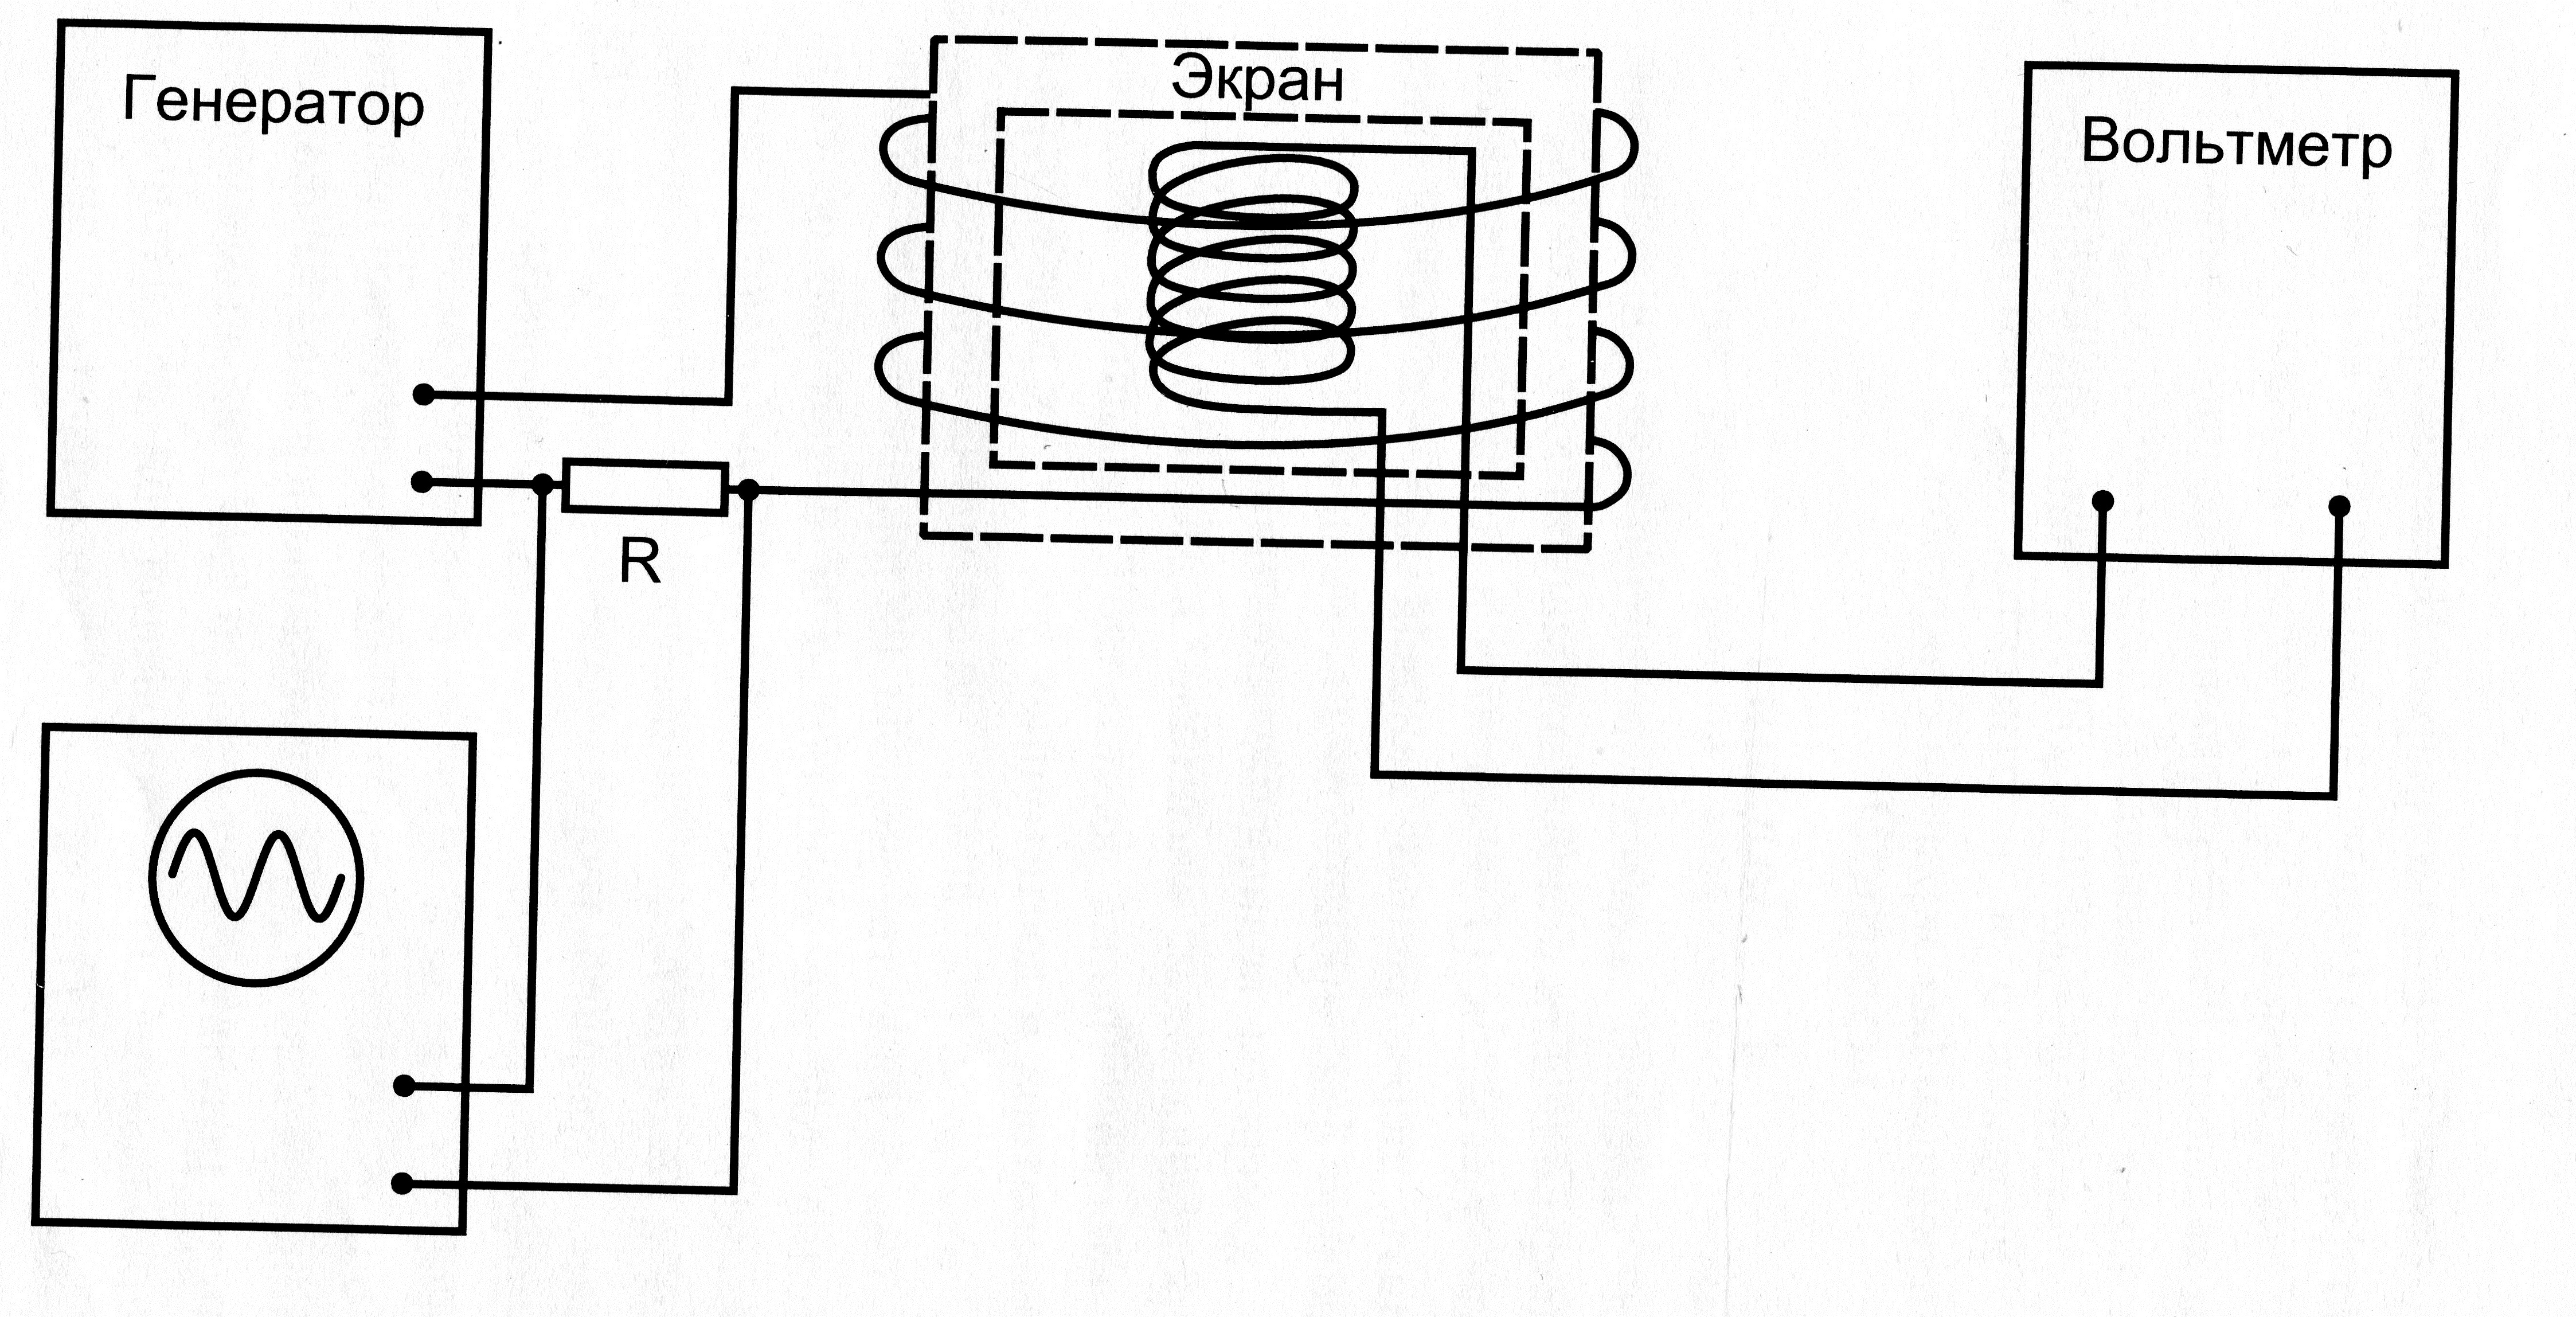
\includegraphics[width = 0.9\linewidth]{imgs/graphs/img744.jpg}
    \caption{Схема установки}
    \label{fig:1}
\end{figure}

Переменное магнитное поле создается внутри соленоида, подключенного к выходу звукового генератора. В качестве индикатора поля используется второй соленоид, с выхода которого переменное напряжение может подаваться на усилитель вольтметра. Надевая больший (генераторный) соленоид сначала на открытый (неэкранированный) индикатор, а затем на индикатор, закрываемый экраном, и измеряя, как изменяются при этом показания вольтметра, можно (при неизменности амплитуды тока в цепи внешнего соленоида) определить коэффициент ослабления. Поскольку внесение металлического экрана внутрь внешнего соленоида изменяет его коэффициент самоиндукции, а следовательно, и его импеданс, сила тока в цепи внешнего соленоида и создаваемое этим током магнитное поле $\vH_0$ при наличии экрана и в его отсутствие могут быть различными. Это нужно учитывать. В используемой схеме предусмотрено измерение относительных изменений токов как во внутреннем, так и во внешнем соленоидах. С этой целью в цепь внешнего соленоида введено сопротивление $R$, напряжение с которого подается на вертикальный усилитель осциллографа. Тогда:
\begin{equation}
 	|\eta_m|=\frac{V_0U_e}{V_eU_0},
	\label{eq:7}
\end{equation}
где V и U - соответственно показания вольтметра и осциллографа, индексы o и e относятся соответственно к величинам, измеренным без экрана и с экраном. 

% В качестве индикатора поля используется второй соленоид меньших размеров (индикаторный), с выхода которого переменное напряжение подается на усилитель вольтметра. 

% Надевая генераторный соленоид сначала на неэкранированный индикаторный, а затем на индикаторный соленоид, закрываемый экраном, и измеряя, как изменяются при этом показания вольтметра, можно по ним вычислить коэффициент ослабления $|\eta_m|$. Кроме этого, необходимо также измерять амплитуду напряжения на осциллографе, подключенного к сопротивлению, которое стоит последовательно генераторному соленоиду.

% \subsection{Учет в $|\eta_m|$ искажения $L_{gen}$ экраном}

% Поле в соленоиде пропорционально току, который в нем течет: $H\sim I$ (это нетрудно вывести на примере бесконечного соленоида с непрерывной обмоткой). Прикладывая к генераторному соленоиду напряжение постоянной амплитуды $u_0$, мы получаем
% \begin{equation}
% 	u_0=Z\cdot I=i\omega L\cdot I \quad\Rightarrow\quad H_{ext}\sim \frac{u_0}{\omega L}
% \end{equation}

% Когда мы измеряем напряжение на индикаторном соленоиде, находящемся в поле $H_{in}$, оно равно 
% \begin{equation}
% 	V=i\omega L_{ind}\cdot I_{ind} \sim \omega  L_{ind} H_{in}
% \end{equation}

% Индуктивность индикаторного соленоида не зависит от наличия экрана, поэтому
% \begin{equation}
% 	\frac{H_{in}^{(0)}}{H_{in}^{(e)}}=\frac{V_0}{V_e},
% \end{equation}
% где $H_{in}^{(0)}$ -- поле в индикаторном соленоиде без надетого экрана, $H_{in}^{(e)}$ -- поле в индикаторном соленоиде с надетым экраном.

% Очевидно, поле $H_{in}^{(0)}=H_{ext}^{(0)}$. Но поле $H_{in}^{(e)}$ -- это не ослабленное поле $H_{ext}^{(0)}$, потому что при внесении экрана в генераторный соленоид $H_{ext}=H_{ext}^{(e)}=H_{ext}^{(0)}\cdot\frac{L_0}{L_e}$, где $L_0$ -- индуктивность генераторного соленоида без экрана, $L_e$ -- с экраном.

% Значит, если бы при внесенном экране генераторный соленоид создавал поле $H_{ext}^{(0)}$, то внутри экрана бы было поле $H_{in}^{(e)}\cdot\frac{L_e}{L_0}$ (в линейном приближении).

% Отсюда следует, что
% \begin{equation}
% 	|\eta_m|=\frac{H_{ext}^{(0)}}{H_{in}^{(e)}\cdot\frac{L_e}{L_0}}=\frac{V_0}{V_e}\cdot\frac{L_0}{L_e}
% \end{equation}

% Так как мы измеряем напряжение $U$ на резисторе в цепи генераторного соленоида (допустим, что резистор не искажает импеданс: $R\ll \omega L$)

% \begin{equation}
% 	U_e=I_eR, \quad\Rightarrow\quad L_e\sim \frac{u_0}{\omega I_e}=\frac{u_0 R}{\omega U_e}
% \end{equation}
% С другой стороны, 
% \begin{equation}
% 	L_0\sim \frac{u_0}{\omega I_0} = \frac{u_0 R}{\omega U_0}
% \end{equation}
% Тогда окончательно
% \begin{equation}
% 	|\eta_m|=\frac{V_0U_e}{V_eU_0}
% \label{eq:7}
% \end{equation}
% где $V$ и $U$ - соответственно показания вольтметра и осциллографа, индексы $0$ и $e$ относятся соответственно к величинам измеренным без экрана и с экраном.


\newpage
\section{Экспериментальные результаты}
\subsection{Измерение $|\eta_m|$ латунных и стальных экранов}

При измерении каждого экрана производилась подстройка напряжения на генераторном соленоиде, чтобы оно было одно и тоже при отсутствии экрана и его внесении, чтобы можно было применять формулу \eqref{eq:7}.

\begin{table}[h!]
	\caption{Измерение экранирования латунными экранами}
	\label{tab:6s1}
	\vspace{1em}
	\centering
	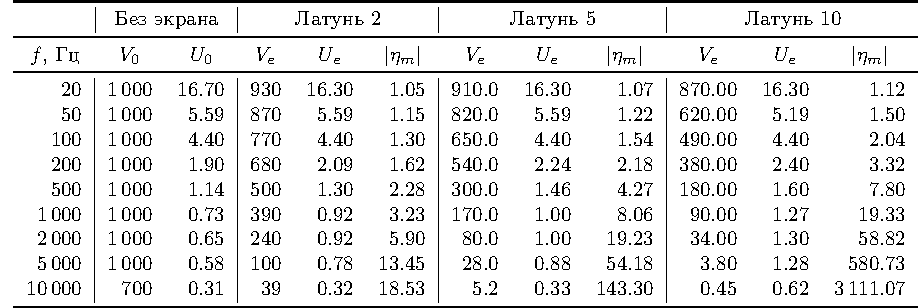
\includegraphics[width=\textwidth]{tables/table1}
\end{table}

У стальных экранов некоторые измерения не были произведены полностью, ввиду сильного падения $V_e$ и появления шумов, искажающих результаты (шум больше точности измерения).

\begin{table}[h!]
	\caption{Измерение экранирования стальными экранами}
	\label{tab:6s1}
	\vspace{1em}
	\centering
	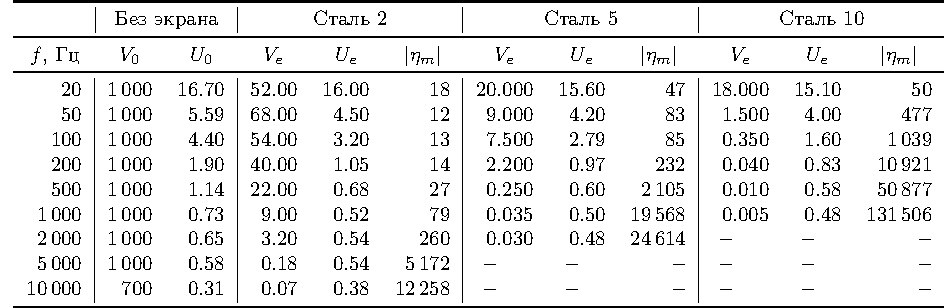
\includegraphics[width=\textwidth]{tables/table2}
\end{table}

Для полученных результатов по всем частотам и всем экранам рассчитан $|\eta_m|$ и построены графики в логарифмическом масштабе по обеим осям.

На рисунке \ref{fig:all} (см. стр. \pageref{fig:all}) приведены шесть графиков для каждого экрана. 

\begin{figure}[H]
	% \vspace{-15pt}
	\centering
	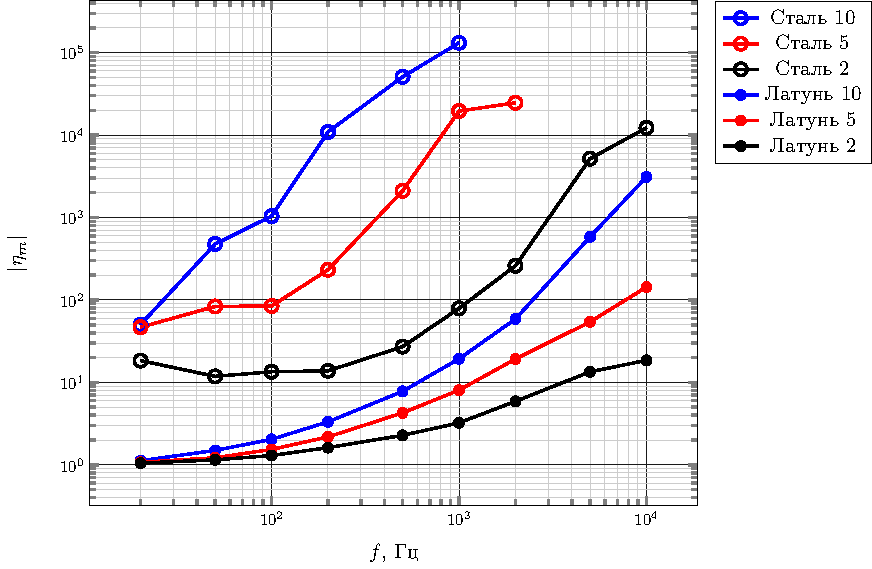
\includegraphics[scale=1]{imgs/graphs/eta}
	\caption{Результаты эксперимента для трех латунных и трех стальных экранов}
	\label{fig:all}
\end{figure}

\subsection{Совмещение теории и эксперимента для латунных экранов}

\begin{figure}[H]
	% \vspace{-10pt}
	\centering
	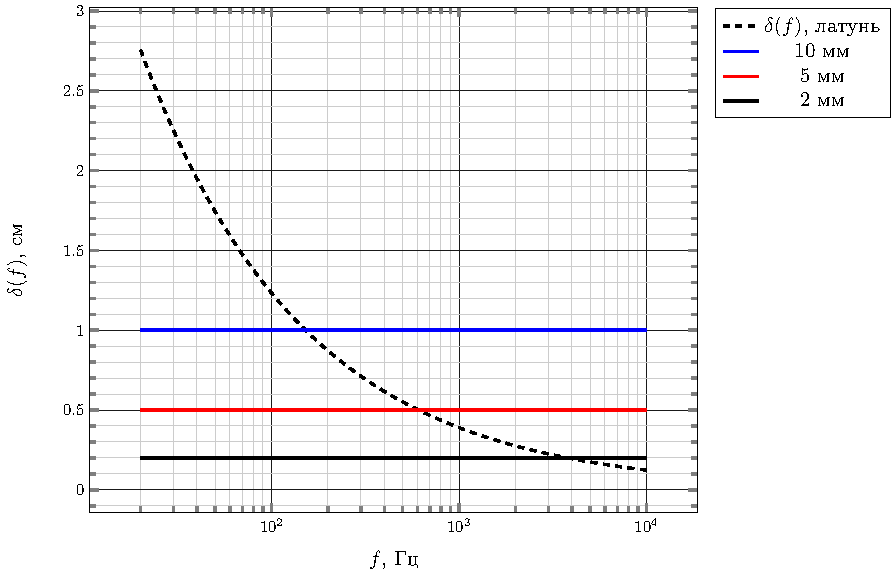
\includegraphics[scale=1]{imgs/graphs/delta}
	\caption{Разграничение применимости формул толщиной скин-слоя $\delta(f)$}
	\label{fig:figure3}

\end{figure}
\begin{figure}[H]
	% \vspace{-10pt}
	\centering
	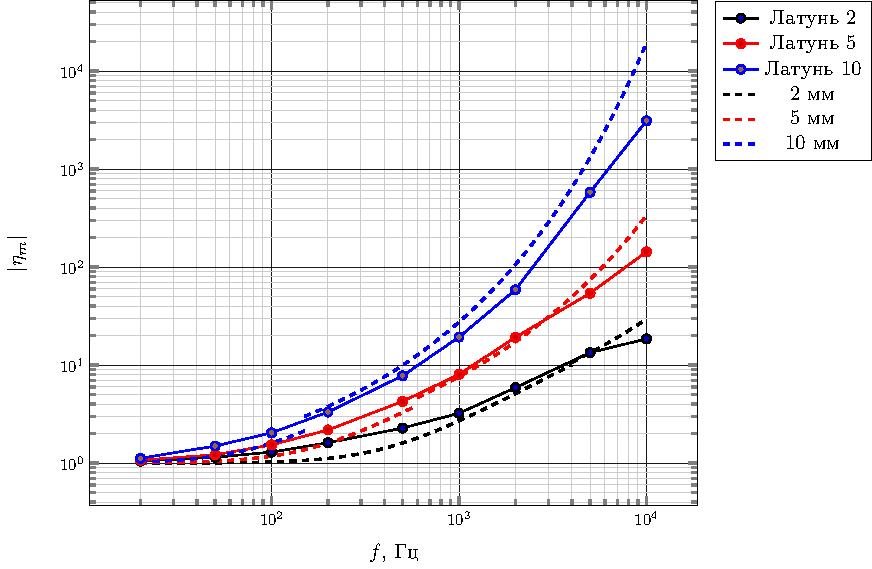
\includegraphics[scale=1]{imgs/graphs/eta_wt}
	\caption{Наложение теоретических графиков (пунктиром) на экспериментальные для латунных экранов}
	\label{fig:figure3}
	% \vspace{-10pt}
\end{figure}
Принимая в качестве модели цилиндрического экрана сферический слой той же толщины $d$ и с тем же объемом внутренней полости $V=(4\pi/3)(a-d)^3=\pi R^2h$ (отсюда, ввиду $a\gg d$, имеем $a\cong (3R^2h/4)^{1/3}$), построили для исследуемых экранов графики теоретической зависимости $|\eta_m(f)|$.

Для разграничения области применения формул различных приближений по $\delta/d$, построен график $\delta(f)$ для латуни и на нем построены константы $d=0.2,0.5,1.0$ см.  

Хорошее качественное совпадение наблюдается в области частот до 6 кГц. Для более высоких частот теоретические кривые нарастают быстрее с ростом частоты.

% \newpage
\subsection{Оценка $\mu$ для стальных экранов по результатам измерений}

Для стальных экранов почти всюду выполняется $\delta \ll d$, поэтому оценка производится из формулы

\begin{gather}
	\eta_m = \frac16\qty[(1-i)\frac{\mu \delta}{a} + 3 + (1+i)\frac{a}{\mu \delta}]\exp\qty[(1+i)\frac{d}{\delta}]
\end{gather}

Взяв модуль от этого выражения, получим:
\begin{gather}
	|\eta_m| = \frac{\exp\qty[\frac{d}{\delta}]}{6}\sqrt{\qty(\frac{\mu \delta}{a} +3 + \frac{a}{\mu \delta} )^2 + \qty(\frac{a}{\mu \delta} - \frac{\mu \delta}{a})^2}
\end{gather}

Здесь можно получить итерационное уравнение для $\mu$ двумя способами: через логарифмирование и приведение к общему знаменателю. Для начала приведем формулу к общему знаменателю:

\begin{gather}
	|\eta_m| = \frac{\exp\qty[\frac{d}{\delta}]}{6 \mu \delta a}\sqrt{\qty((\mu \delta)^2 +3 a \mu \delta + a^2)^2 + \qty(a^2 - (\mu \delta)^2)^2}\\
%
	\mu = \frac{\exp\qty[\frac{d}{\delta}]}{6 |\eta_m| \delta a}\sqrt{\qty((\mu \delta)^2 +3 a \mu \delta + a^2)^2 + \qty(a^2 - (\mu \delta)^2)^2}
\end{gather}

% Теперь перенесем экспоненту в левую часть и прологарифмируем:

% \begin{gather}
% 	\exp\qty[\frac{-d}{\delta}] = \frac{1}{6 \mu \delta a |\eta_m|}\sqrt{\qty((\mu \delta)^2 +3 a \mu \delta + a^2)^2 + \qty(a^2 - (\mu \delta)^2)^2}\\
% %
% 	\frac{-d}{\delta} = \ln \qty{\frac{1}{6 \mu \delta a |\eta_m|}\sqrt{\qty((\mu \delta)^2 +3 a \mu \delta + a^2)^2 + \qty(a^2 - (\mu \delta)^2)^2}}\\	
% \end{gather}

% Осталось подставить $\delta = \frac{c}{\sqrt{2\pi\sigma \mu \omega}}$ и выразить $\mu$

% \begin{gather}
% 	\mu = \frac{c^2}{d^2 2\pi\sigma\omega} \ln\qty{\frac{6a|\eta_m|c\sqrt{\mu}}{\sqrt{2\pi\sigma\omega}} \cdot \qty( \qty(\frac{\mu c^2}{2\pi\sigma \omega} + \frac{3a\sqrt{\mu} c}{\sqrt{2\pi\sigma\omega}} + a^2)^2 + \qty(a^2 - \frac{c^2\mu}{2\pi\sigma \omega})^2 )^{-1/2}}
% \end{gather}

Эту формулу можно представить (зафиксировав $\omega$ и взяв из эксперимента $|\eta_m(\omega)|$) в виде
\begin{equation}
	\mu=F(\mu)
\end{equation}

Это уравнение в виде, пригодном для применения известного метода простых итераций, который заключается в задании начального приближения $\mu^{(0)}$ и итерационного процесса:
\begin{equation}
	\mu^{(1)}=F(\mu^{(0)}),\quad
	\mu^{(2)}=F(\mu^{(1)}),\quad
	\mu^{(3)}=F(\mu^{(2)}),\quad\ldots
\end{equation}

Начальное приближение можно выбрать из диапазона $\mu=10^2 \divisionsymbol 10^3$.

Хотя функция, стоящая справа, на самом деле не удовлетворяет условиям устойчивости (сходимости) численного решения, но все равно можно найти этим методом решение, перебирая начальные значения $\mu$ до того значения, когда точка меняет направление расходимости. 

Для 2 мм -- стали полученное таким методом значение на частоте $500$ Гц дает $\mu=153$. На графике (см. рис \ref{fig:eta_wt_steel}, стр.\pageref{fig:eta_wt_steel}) хорошо видно, что действительно это значение дает численное решение этого уравнения, и теоретический график проходит через практическую точку.

Для 5 мм -- стали (на частоте 500 Гц) $\mu=140$, для 10 мм -- стали (на частоте 200 Гц) $\mu=130$.

Экспериментальные точки подбирались таким образом, чтобы рассчитанная из них $\mu$ давала теоретические графики, наиболее хорошим образом описывающие экспериментальные кривые, хотя бы в диапазоне не очень больших частот.


Расхождение теоретического графика (который уходит в значительно большие по сравнению с практическими $|\eta_m|$)  и практического, который перестает расти, можно объяснить частотным насыщением магнитной проницаемости стали: доменная структура не успевает изменяться вслед за частотой поля, и $\mu$ начинает падать с ростом частоты.

\begin{figure}[H]
	\centering
	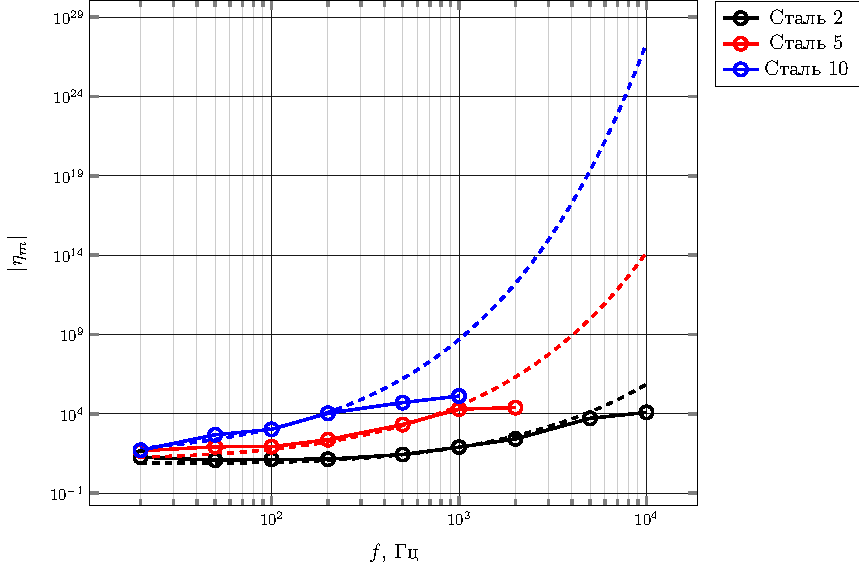
\includegraphics[scale=1]{imgs/graphs/eta_wt_steel}
	\caption{Сопоставление теоретических графиков и практических для стальных экранов}
	\label{fig:eta_wt_steel}
\end{figure}

% \end{document}


























 














































% Используя результаты измерений для стальных экранов, рассчитали приблизительно на основании той же сферической модели для случая $\delta (f) \ll d$ (формула \eqref{eq:2}) значения магнитной проницаемости стали $\mu$. Способ приближенного расчета состоял в численном решение уравнения для 3 нижних частот (для высоких частот модель \textbf{не совпадает}) частот и последующем усреднении результатов.
% \begin{table}[htbp]
%   \centering
%   \caption{Магнитная проницаемость $\mu$ для разных частот $f$ и толщины экрана $d$}
%     \begin{tabular}{|c|c|c|c|}
%     \toprule
%     $f$, Hz & $\mu$, 2mm & $\mu$, 5mm & $\mu$, 10mm \\
%     \midrule
%     20 & 306.25 & 13.05 & 18.64 \\
%     \midrule
%     50 & 179.35 & 38.76 & 32.26 \\
%     \midrule
%     100 & 94.83 & 102.01 & 146.13 \\
%     \midrule
%     $\langle \mu \rangle$ & 193.48 & 51.27 & 65.68 \\
%     \bottomrule
%     \end{tabular}%
% \end{table}%
% По полученным данным можно сделать вывод о недостаточной точности эксперимента. Хотя качественно $\mu$ для стали действительно лежит в пределах $100-1000$.
\section{Результаты}
% \begin{enumerate}
	В работе было исследовано явление экранирования переменного магнитного поля стальными и латунными экранами. 

	Произведен расчет и сопоставление экранирующих свойств латунных экранов с экспериментальными с помощью модели сферического слоя. Выявлено хорошее совпадение теории с практикой до $f=6$ кГц. 

	Численными методами найдены $\mu$ для стальных экранов, дающие наиболее адекватное соответствие теоретических графиков практическим: $\mu=153,140,130$ для 2,5,10 мм экранов. В этом случае теория дает качественное соответствие вплоть на частотах $f \simeq 1$ кГц.
% \end{enumerate}


\begin{thebibliography}{}
	\bibitem{met} Гильденбург В.Б., Павличенко И.А. Практикум: электромагнитное экранирование. --- Н. Новгород: ННГУ, 2016. --- 20 с.
\end{thebibliography}
\end{document}
